% !TEX root = QlockToo.tex
% Software
\section{Software}
\label{sec:Software}

\begin{figure}[t]
    \centering
    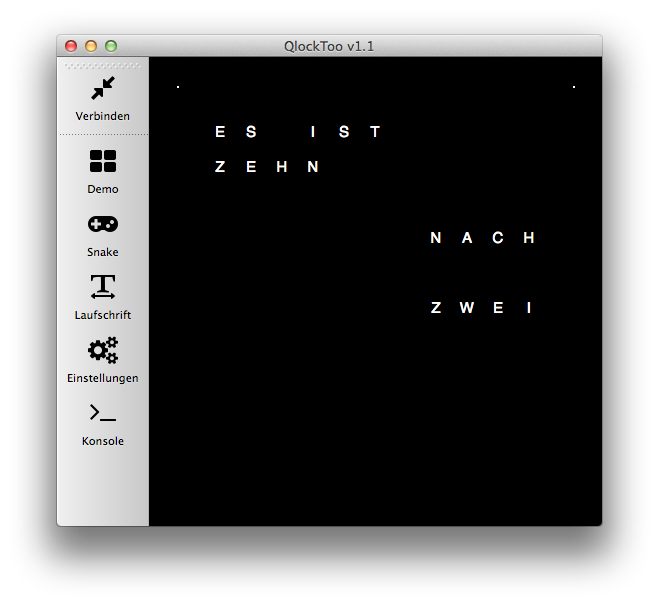
\includegraphics[width=.7\textwidth]{Abbildungen/Software/Manager02}
    \caption[QlockToo-Manager]{Der QlockToo-Manager}
    \label{fig:Manager}
\end{figure}

\begin{multicols}{2}
Im ersten Projektschritt zur Entwicklung der Uhr wird eine Desktop-Software, der QlockToo-Manager, programmiert, welche den Testprozess der Algorithmen deutlich beschleunigt. Mit weiterem Projektfortschritt wächst auch der Programmumfang. Durch stetige Weiterentwicklung kommen zahlreiche Funktionen hinzu, welche im folgenden dargestellt sind:

\begin{itemize}

\item Die Software enthält einen Simulator. Dieser stellt alle Muster und Algorithmen direkt ohne Anschluss an die Hardware dar.
\item Zu Testzwecken sind verschiedene Demonstrationsmuster implementiert.
\item Mit Hilfe einer Laufschrift können frei wählbare Texte in beliebiger Geschwindigkeit angezeigt werden.
\item Das Handyspiel Snake kann auf dem Uhrenschirm gespielt werden. Die Steuerung erfolgt über die Pfeiltasten am Computer.
\item Über eine USB-Schnittstelle fungiert die QlockToo als Display der Software. Das notwendige Streaming-Protokoll wird eigens für diese Anwendung entwickelt.
\item Zur Einstellung der QlockToo über den Computer ist ein Einstellungsdialog implementiert. Dieser ermöglicht zusätzliche Einstellmöglichkeiten über die Funktionen der vier Tasten hinaus.
\end{itemize}

\subsection{Aufbau}
Um eine Lauffähigkeit auf allen gängigen Plattformen (Windows / Mac OS X / Linux) zu realisieren wird die Programmiersprache Python verwendet. Weiterer Vorteil ist die hohe Entwicklungsgeschwindigkeit.
Das aus der C++ - Welt bekannte Framework Qt wird über die von Digia bereitgestellten PySide-Bindings als GUI-Framework genutzt. Die Software baut somit ausschließlich auf freier Open-Source Software auf.

\subsection{Simulator}
Der QlockToo-Manager zeigt nach dem Start den Simulator. Seitlich wird eine Menüleiste zum Starten der Unterprogramme dargestellt.
Solange kein Unterprogramm ausgewählt ist, wird standardmäßig das Programm \emph{Timewords}, welches für die Anzeige der Zeit in Worten zuständig ist, angezeigt. Der QlockToo-Manager bedient sich dazu der momentanen Systemzeit.

Die Unterprogramme sind jeweils einzelne, voneinander unabhängige Python-Module. Eine Erweiterung ist somit jederzeit möglich.

Der Simulator besitzt die gleiche API wie die Hardware. Die Ausgabe der Programme kann somit ohne Anpassungen auf die Hardware gestreamt oder im Simulator angezeigt werden. Auch eine parallele Darstellung ist möglich.
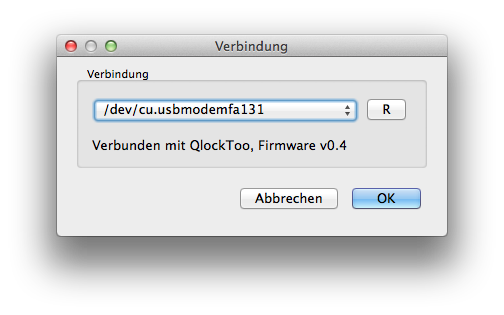
\includegraphics[width=\columnwidth]{Abbildungen/Software/ConnectDialog}

Im Entwicklungsmodus ist eine Konsole integriert, mit der direkt Befehle an die API der QlockToo gesendet werden können. Kommandos und Rückgabewerte werden zur einfacheren optischen Erfassung farblich hervorgehoben.

{
    \centering
    \includegraphics[width=0.85\columnwidth]{Abbildungen/Software/Linux}
}


\subsection{Demonstrationsmuster}
Der zweite Punkt in der Menüleiste sind die Demonstrationsmuster. Zur besseren Sichtbarkeit sind die Muster invertiert dargestellt. Folgende Demonstrationen stehen zur Verfügung:

\textbf{Pulse}
Alle LEDs wechseln sanft zwischen minimaler und maximaler Helligkeit.

\textbf{Fade}
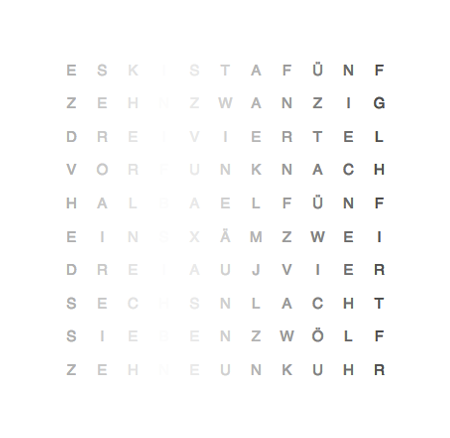
\includegraphics[width=\columnwidth]{Abbildungen/Software/Demo/Fade}
Ein Farbverlauf bewegt sich sinusförmig von links nach rechts und zurück.

\textbf{Wave}
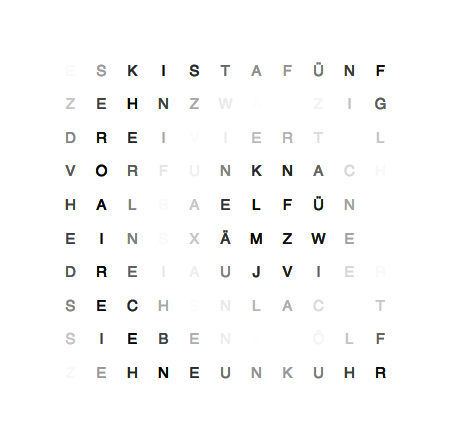
\includegraphics[width=\columnwidth]{Abbildungen/Software/Demo/Welle}
Das Muster Wave zeigt ein pulsierendes Wellenbild, dessen Zentrum mit der Zeit langsam über den Bildschirm wandert.

\textbf{Pixeltest}
Hierbei werden die Pixel einzeln hintereinander beleuchtet. Diese Demo dient hauptsächlich zum Überprüfen der Verkabelung.

\textbf{Helix}
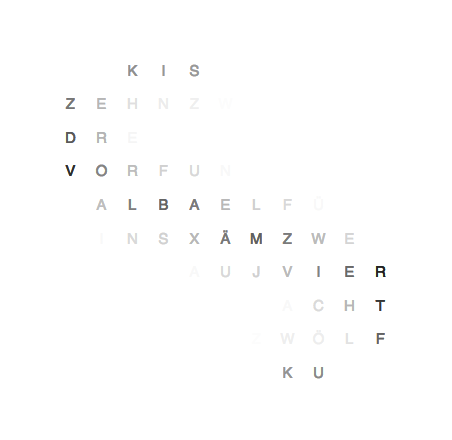
\includegraphics[width=\columnwidth]{Abbildungen/Software/Demo/Helix}
Die Helix-Darstellung zeigt die zweidimensionale Projektion einer dreidimensionalen Spirale. Die z-Achse wird dabei über unterschiedliche Helligkeitswerte visualisiert.
Bedingt durch die Berechnung der Funktionswerte für diskrete Buchstaben auf der Uhr und die geringe Pixelanzahl der Uhr wirkt die Demonstration zunächst sehr dünn und zerstückelt. Durch die Implementierung eines Gauss-Tiefpasses, wird der gewünschte Anti-Alias-Effekt erzielt. Die 3D Darstellung ist so sehr viel deutlicher.

\textbf{Game Of Life}
Darstellung von Conways Game of Life, anhand toter (schwarz) und lebender (weiß) Zellen.
Grundlage sind folgende vier Regeln, die bei jeder Iteration befolgt werden\footnote{de.wikipedia.org/wiki/Conways\_Spiel\_des\_Lebens}:
\begin{itemize}
\item Eine tote Zelle mit genau drei lebenden Nachbarn wird in der Folgegeneration neu geboren.
\item Lebende Zellen mit weniger als zwei lebenden Nachbarn sterben in der Folgegeneration an Einsamkeit.
\item Eine lebende Zelle mit zwei oder drei lebenden Nachbarn bleibt in der Folgegeneration lebend.
\item Lebende Zellen mit mehr als drei lebenden Nachbarn sterben in der Folgegeneration an Überbevölkerung.
\end{itemize}

\textbf{Matrix}
Der berühmte Effekt aus dem Wachowski-Film \emph{Matrix} bietet sich wegen des Designs der QlockToo besonders an.
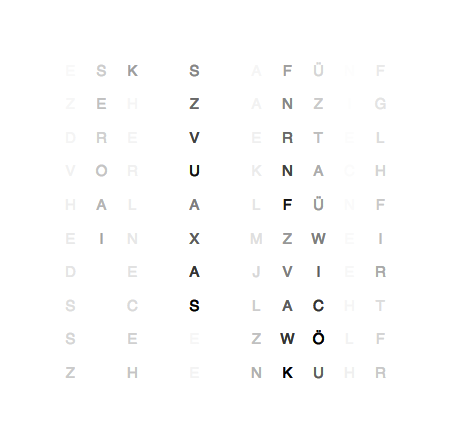
\includegraphics[width=\columnwidth]{Abbildungen/Software/Demo/Matrix}


\end{multicols}

